Most of our system sequence diagrams have been extended to interaction diagrams of system-wide operations. 
An example of this can be seen in figure \ref{fig:merge-ssd}, 
which has laid basis for the interaction diagram depicting the merge process, 
as seen in Appendix \ref{sec:interaction-diagram-appendix} on page \pageref{fig:uc7-interaction-diagram}
The merge operation (figure \ref{fig:merge-ssd}) is a central feature of the \SOP{} 
system, so it has been subject to some revision in the documentation.
The implemented system differs slightly from the diagram, in that the implementation will synchronize all projects at once rather than a document at the time. 
In the implementation, the user is not required to edit conflicting merges either, but rather 
saves the conflicts and lets the user decide when to deal with conflicts.
The diagram is deliberately left in this state, because we agree that it is a better solution, which is simply left out in the proof-of-concept \SOP{} implementation.

\begin{figure}[hbt]
	\centering
	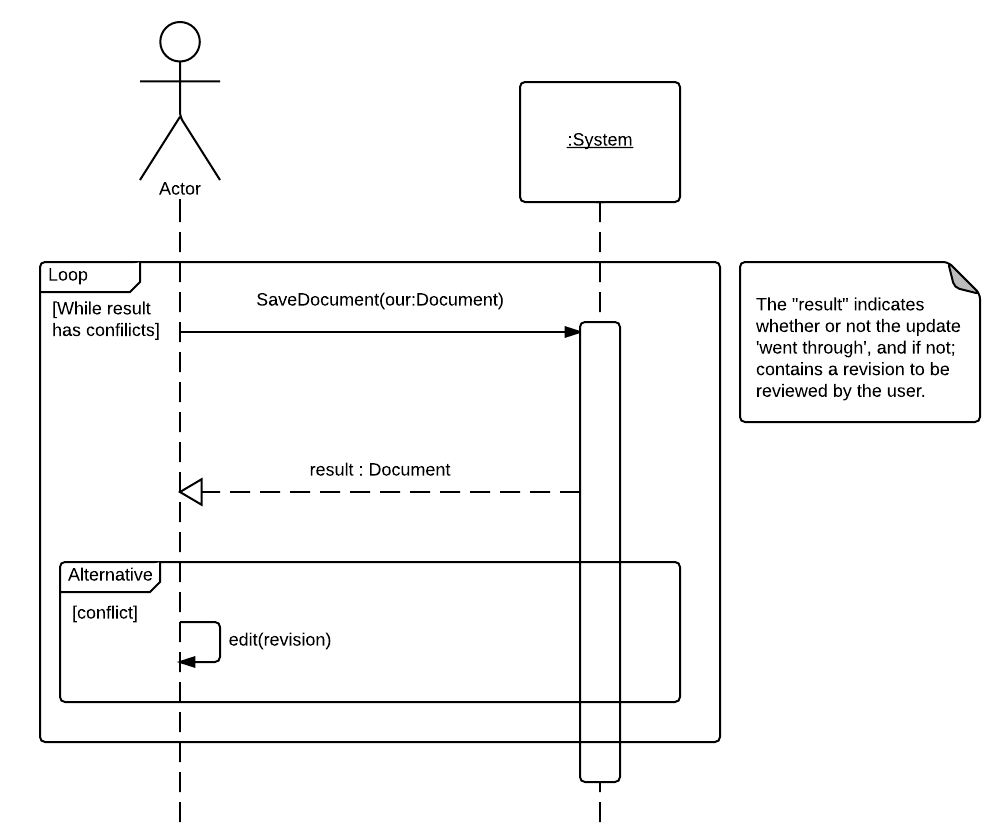
\includegraphics[width=1\textwidth]{Software_analysis/graphics/Merge-ssd.png}
	\caption{A system sequence diagram depicting the merge process}
	\label{fig:merge-ssd}
\end{figure}
